\documentclass[paper=a4,11pt,parskip=half,toc=listof]{scrartcl}
\usepackage{report_package}

\begin{document}
%%%%%%%%%%%%%%%%%%%%% Startseite %%%%%%%%%%%%%%%%%%%%%%%%%%%
\begin{titlepage}
\begin{minipage}[t]{0.5\textwidth}
\begin{Large}
    \begin{flushleft}
      \hspace{1cm} \makebox[3cm][c]{
\includegraphics[height=8ex]{./logos/logo_hbrs.png} \vspace{1.8cm}}
    \end{flushleft}
\end{Large}
\end{minipage}

\vspace{0.07\textheight}
\begin{center}
 \begin{Large} \textbf{\ThesisUniversityCourse} \end{Large}\\
 \vspace{1em}
 \begin{Large} \textbf{-- \ThesisSemester --} \end{Large}\\
 \vspace{2em}
 \begin{Huge} \begin{spacing}{1.3} \textbf{\ThesisTitle} \end{spacing} \end{Huge}
 \vspace{2em}
 \begin{Large} \textbf{-- Report on dataset creation --} \end{Large}\\
 \vspace{2em}
  \begin{Large}\textbf{by} \end{Large}\\
 
 \vspace{2em}
 \begin{Large}\textbf{\ThesisAuthora}\end{Large}\\
 \begin{small}naresh.gurulingan@smail.inf.h-brs.de\end{small}\\
 \begin{small} Matr. no. 9030384\end{small}\\
\end{center}
\end{titlepage}

\newgeometry{top=4cm, bottom=3cm, left=4.5cm, right=3cm}

\newpage
\setcounter{page}{3} 
\begin{spacing}{1.14}
\tableofcontents
\end{spacing}

\clearpage{}
\listoftables % add list of tables
\clearpage{}
\listoffigures % add list of figures 
\clearpage{}
\include{acronym} % include the acronym thing
\clearpage{}

\setcounter{tocdepth}{4} 
\setcounter{secnumdepth}{4}
\setlength\parindent{0pt}  %indent disabled

\pagenumbering{arabic} % arabic numbers for the main part


\newpage
\section{Overview of the dataset}
Since semantic segmentation using deep learning is framed as a pixelwise classification task, an image of dimensions H$\times$W$\times$C requires a ground truth of dimensions H$\times$W, where H and W are the height and width of the image in the dataset having C number of channels. 

The scope of the dataset is to include objects associated to RoboCup @Work. The selected 18 objects are shown in \ref{Fig:1}.

\begin{figure}[!htb]
\centering
\begin{subfigure}{.3\textwidth}
  \centering
  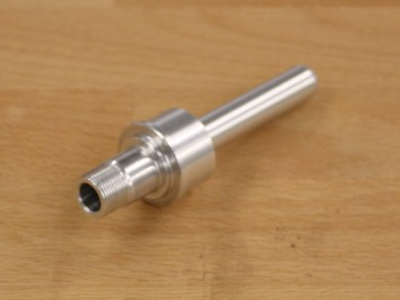
\includegraphics[width=.5\linewidth]{axis}
  \caption{axis \cite{github_robocup@work}}
  \label{fig:axis}
\end{subfigure}%
\begin{subfigure}{.3\textwidth}
  \centering
  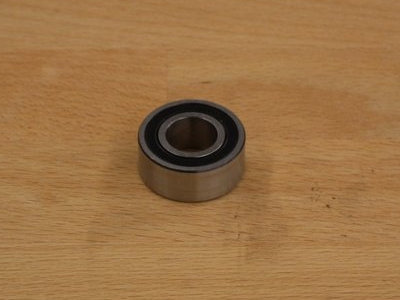
\includegraphics[width=.5\linewidth]{bearing}
  \caption{bearing \cite{github_robocup@work}}
  \label{fig:bearing}
\end{subfigure}
\begin{subfigure}{.3\textwidth}
  \centering
  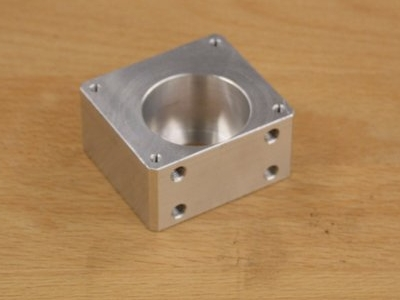
\includegraphics[width=.5\linewidth]{bearingBoxAX01}
  \caption{bearing box AX01 \cite{github_robocup@work}}
  \label{fig:bearingBoxAX01}
\end{subfigure}\\
\vspace{3mm}
\begin{subfigure}{.3\textwidth}
  \centering
  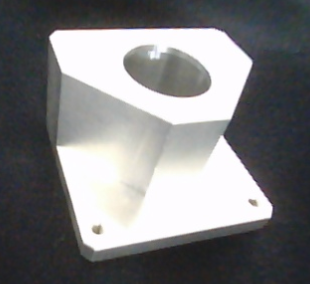
\includegraphics[width=.5\linewidth]{bearingBoxAX16}
  \caption{bearing box AX16}
  \label{fig:bearingBoxAX16}
\end{subfigure}
\begin{subfigure}{.3\textwidth}
  \centering
  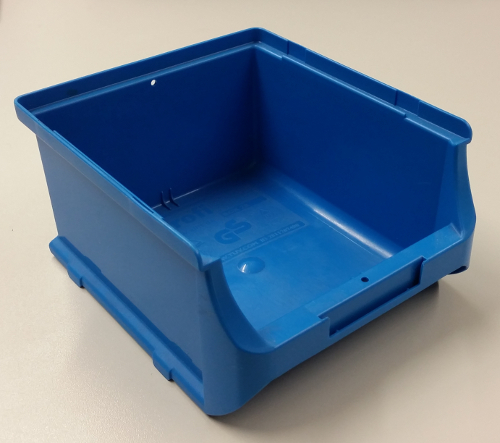
\includegraphics[width=.5\linewidth]{container_blue}
  \caption{container blue \cite{github_robocup@work}}
  \label{fig:container_blue}
\end{subfigure}
\begin{subfigure}{.3\textwidth}
  \centering
  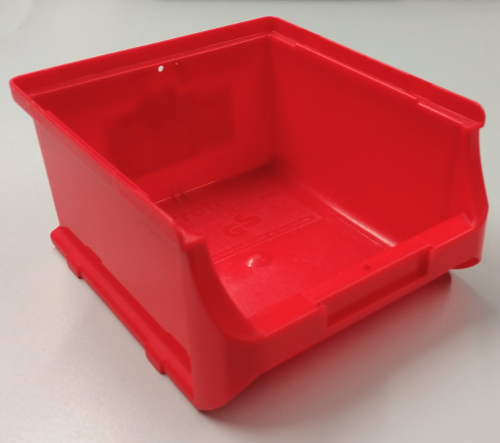
\includegraphics[width=.5\linewidth]{container_red}
  \caption{container red \cite{github_robocup@work}}
  \label{fig:container_red}
\end{subfigure}\\
\vspace{3mm}
\begin{subfigure}{.3\textwidth}
  \centering
  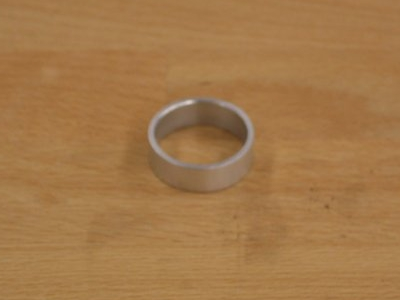
\includegraphics[width=.5\linewidth]{distanceTube}
  \caption{distance tube \cite{github_robocup@work}}
  \label{fig:distanceTube}
\end{subfigure}
\begin{subfigure}{.3\textwidth}
  \centering
  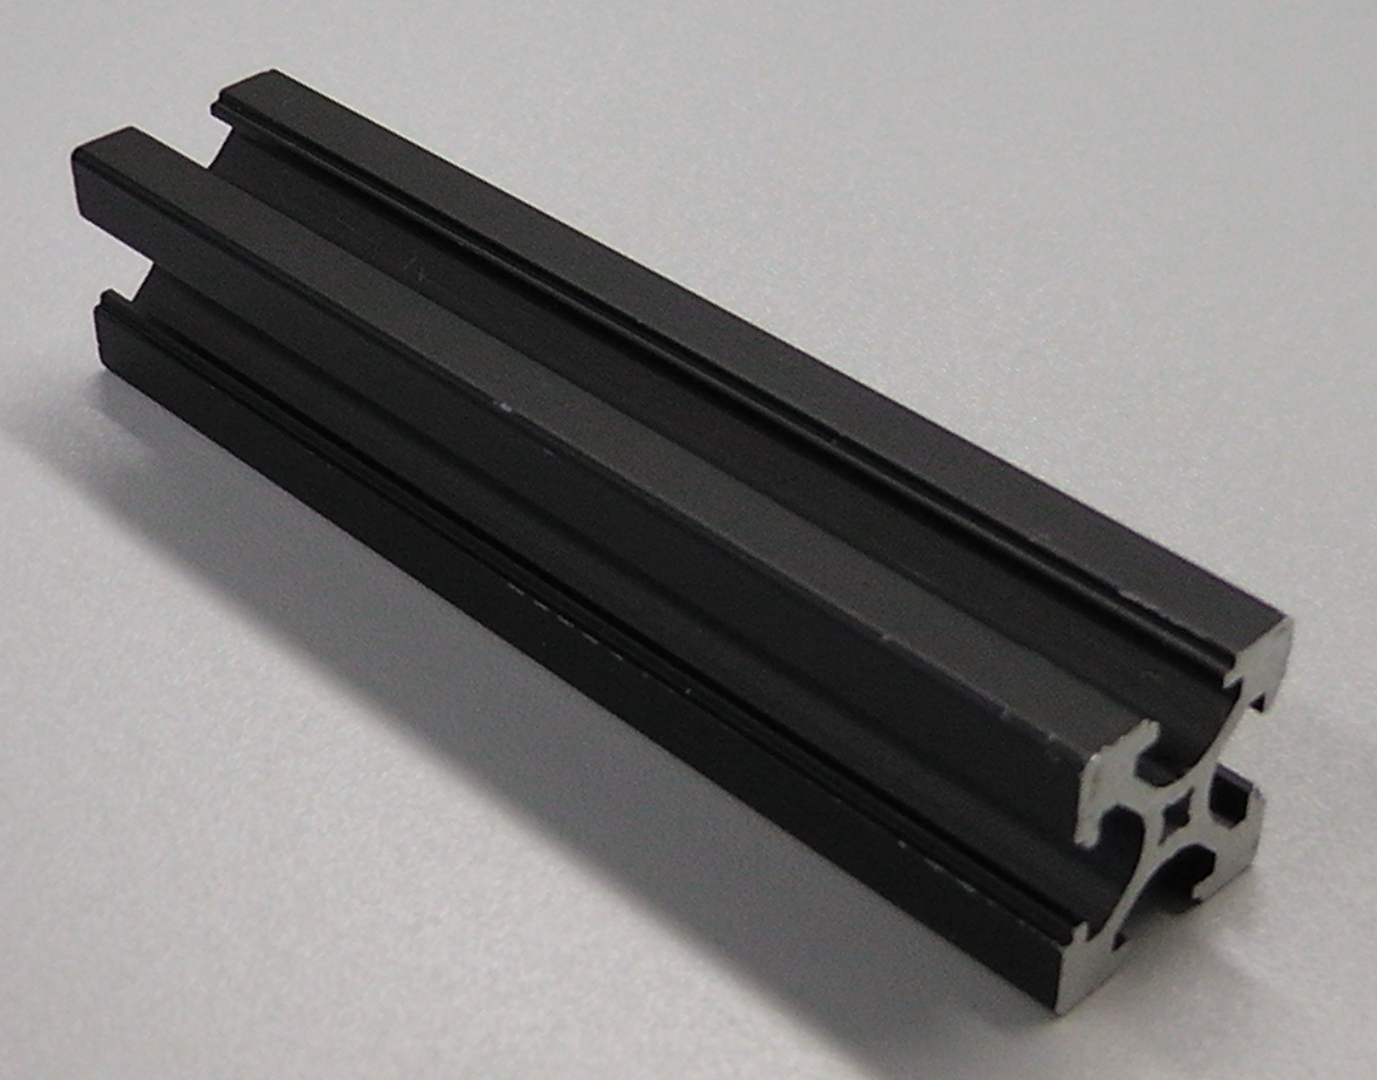
\includegraphics[width=.5\linewidth]{F20_20_B}
  \caption{F20\_20\_B \cite{github_robocup@work}}
  \label{fig:F20_20_B}
\end{subfigure}
\begin{subfigure}{.3\textwidth}
  \centering
  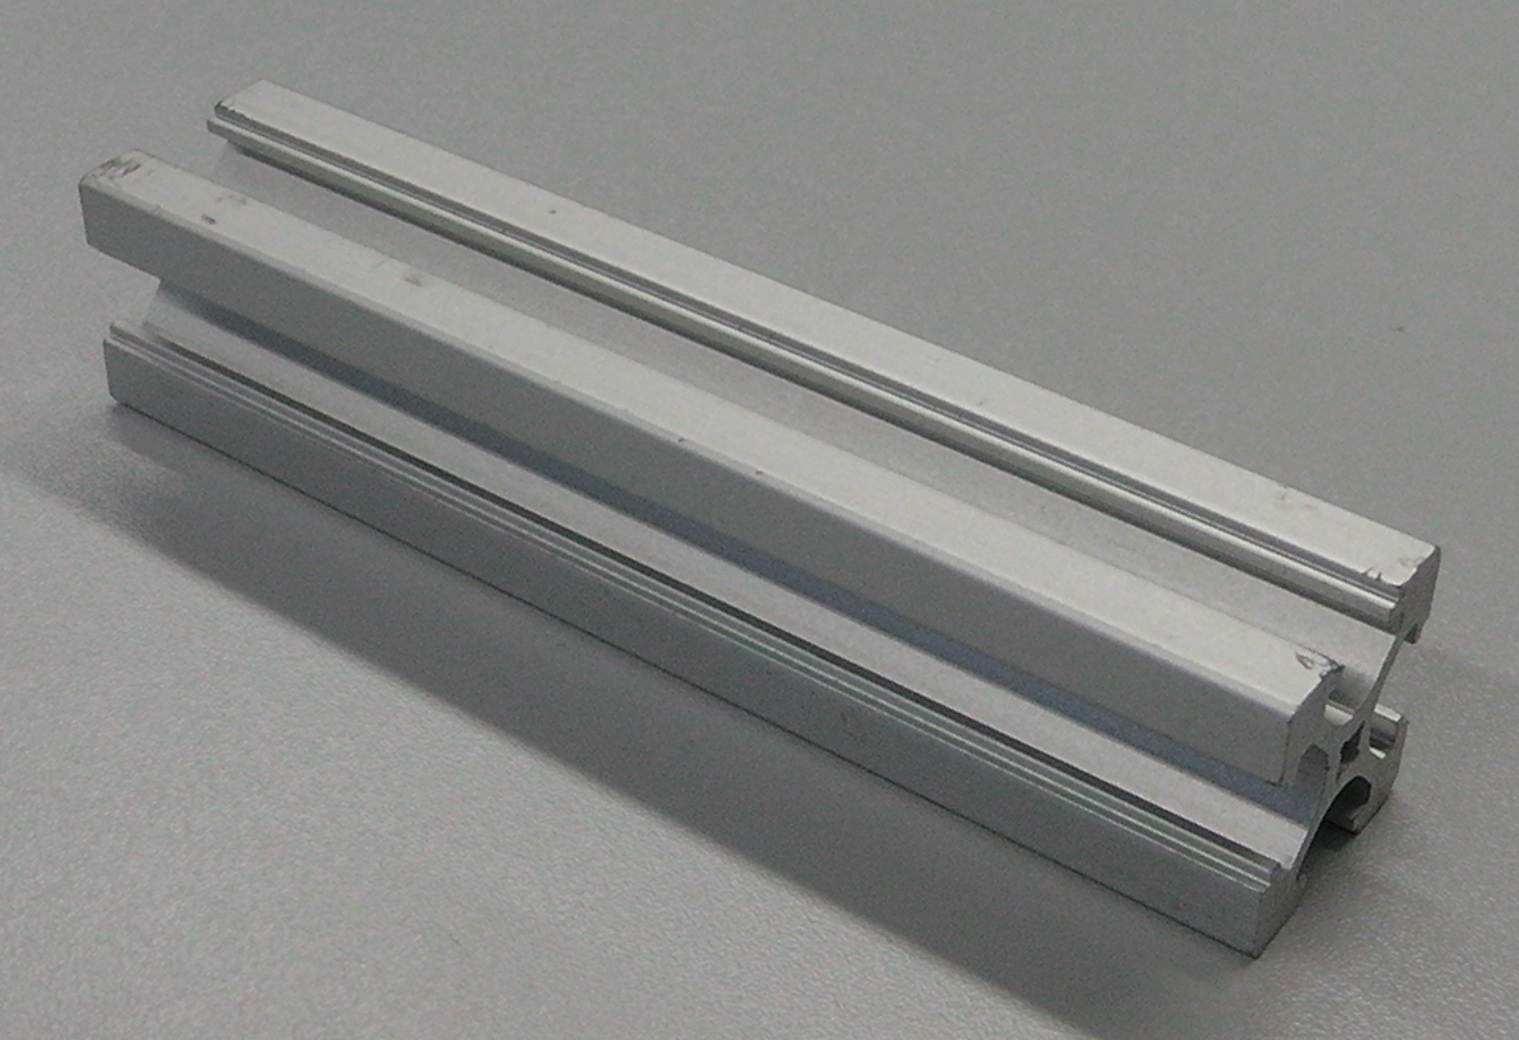
\includegraphics[width=.5\linewidth]{F20_20_G}
  \caption{F20\_20\_G \cite{github_robocup@work}}
  \label{fig:F20_20_G}
\end{subfigure}\\
\vspace{3mm}
\begin{subfigure}{.3\textwidth}
  \centering
  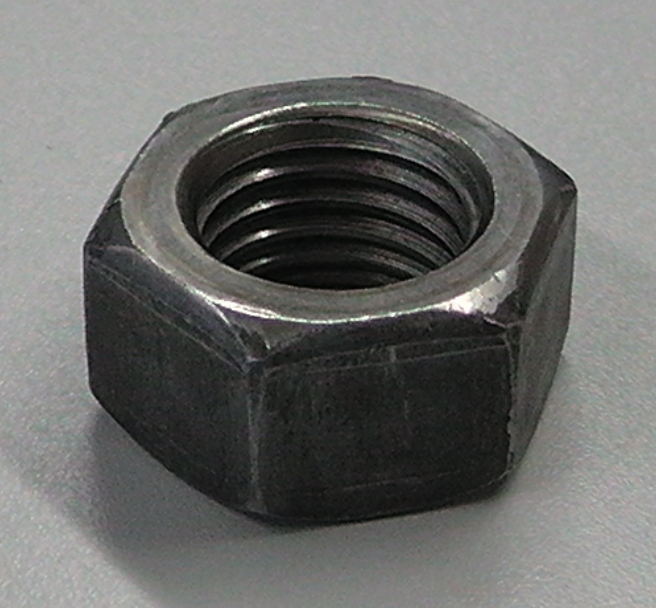
\includegraphics[width=.5\linewidth]{M20}
  \caption{M20 \cite{github_robocup@work}}
  \label{fig:M20}
\end{subfigure}
\begin{subfigure}{.3\textwidth}
  \centering
  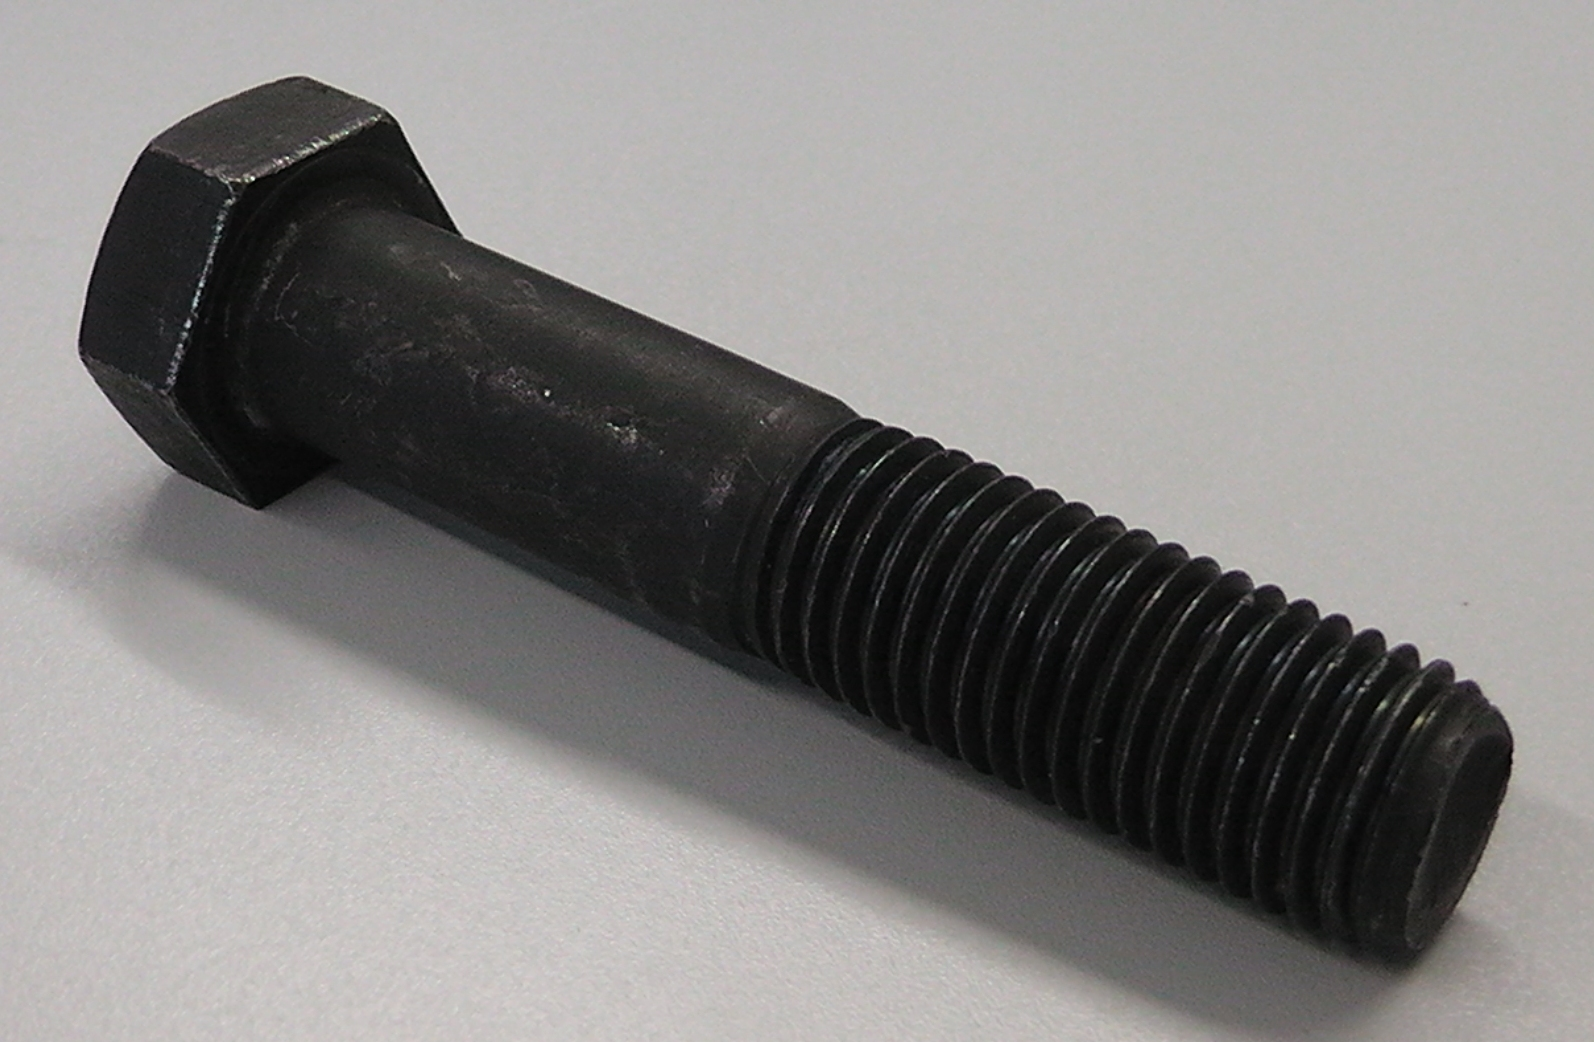
\includegraphics[width=.5\linewidth]{M20_100}
  \caption{M20\_100 \cite{github_robocup@work}}
  \label{fig:M20_100}
\end{subfigure}
\begin{subfigure}{.3\textwidth}
  \centering
  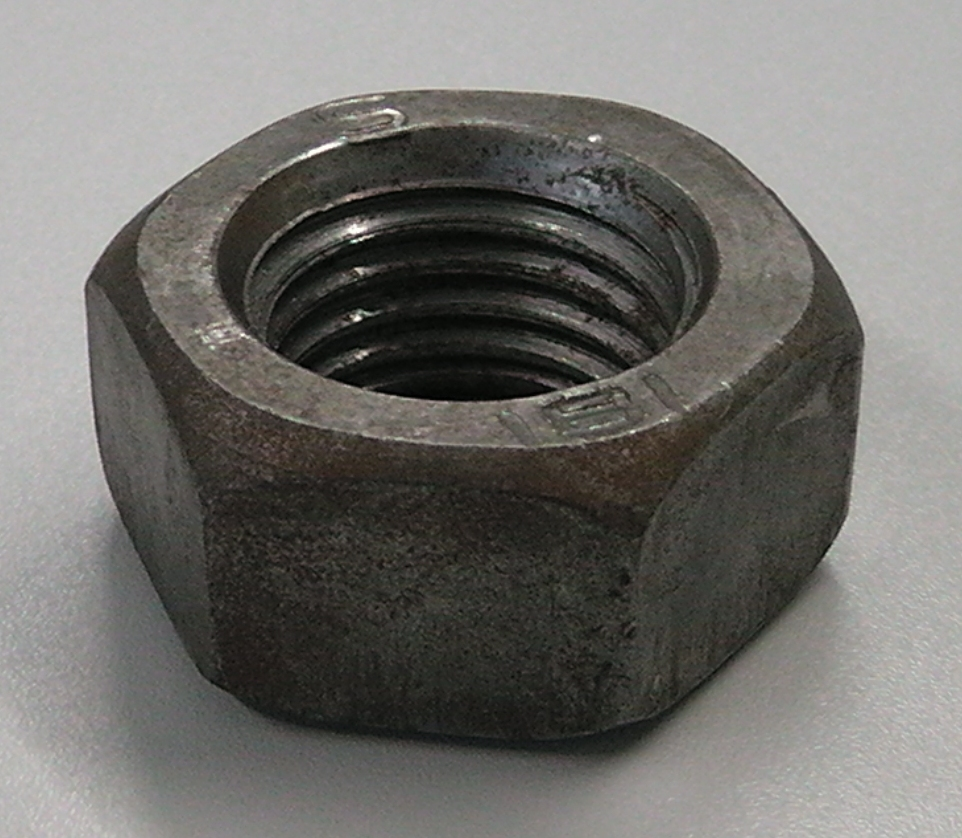
\includegraphics[width=.5\linewidth]{M30}
  \caption{M30 \cite{github_robocup@work}}
  \label{fig:M30}
\end{subfigure}\\
\vspace{3mm}
\begin{subfigure}{.3\textwidth}
  \centering
  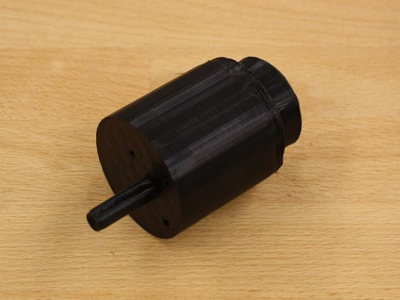
\includegraphics[width=.5\linewidth]{motor}
  \caption{motor \cite{github_robocup@work}}
  \label{fig:motor}
\end{subfigure}
\begin{subfigure}{.3\textwidth}
  \centering
  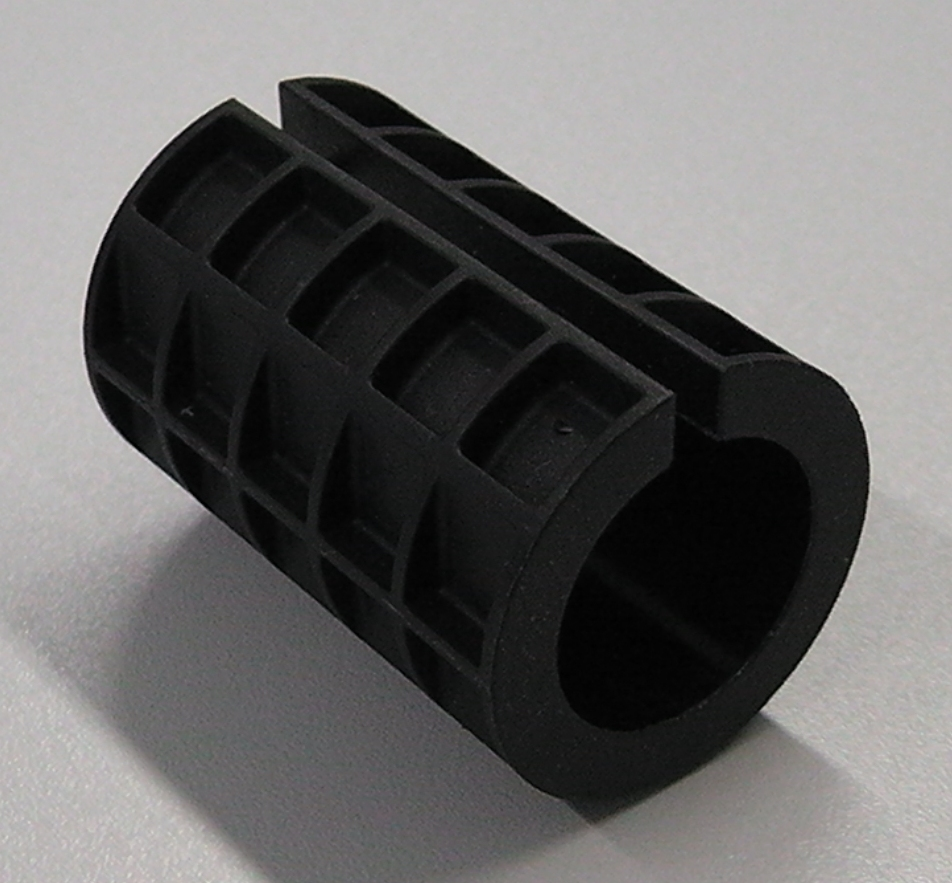
\includegraphics[width=.5\linewidth]{R20}
  \caption{R20 \cite{github_robocup@work}}
  \label{fig:R20}
\end{subfigure}
\begin{subfigure}{.3\textwidth}
  \centering
  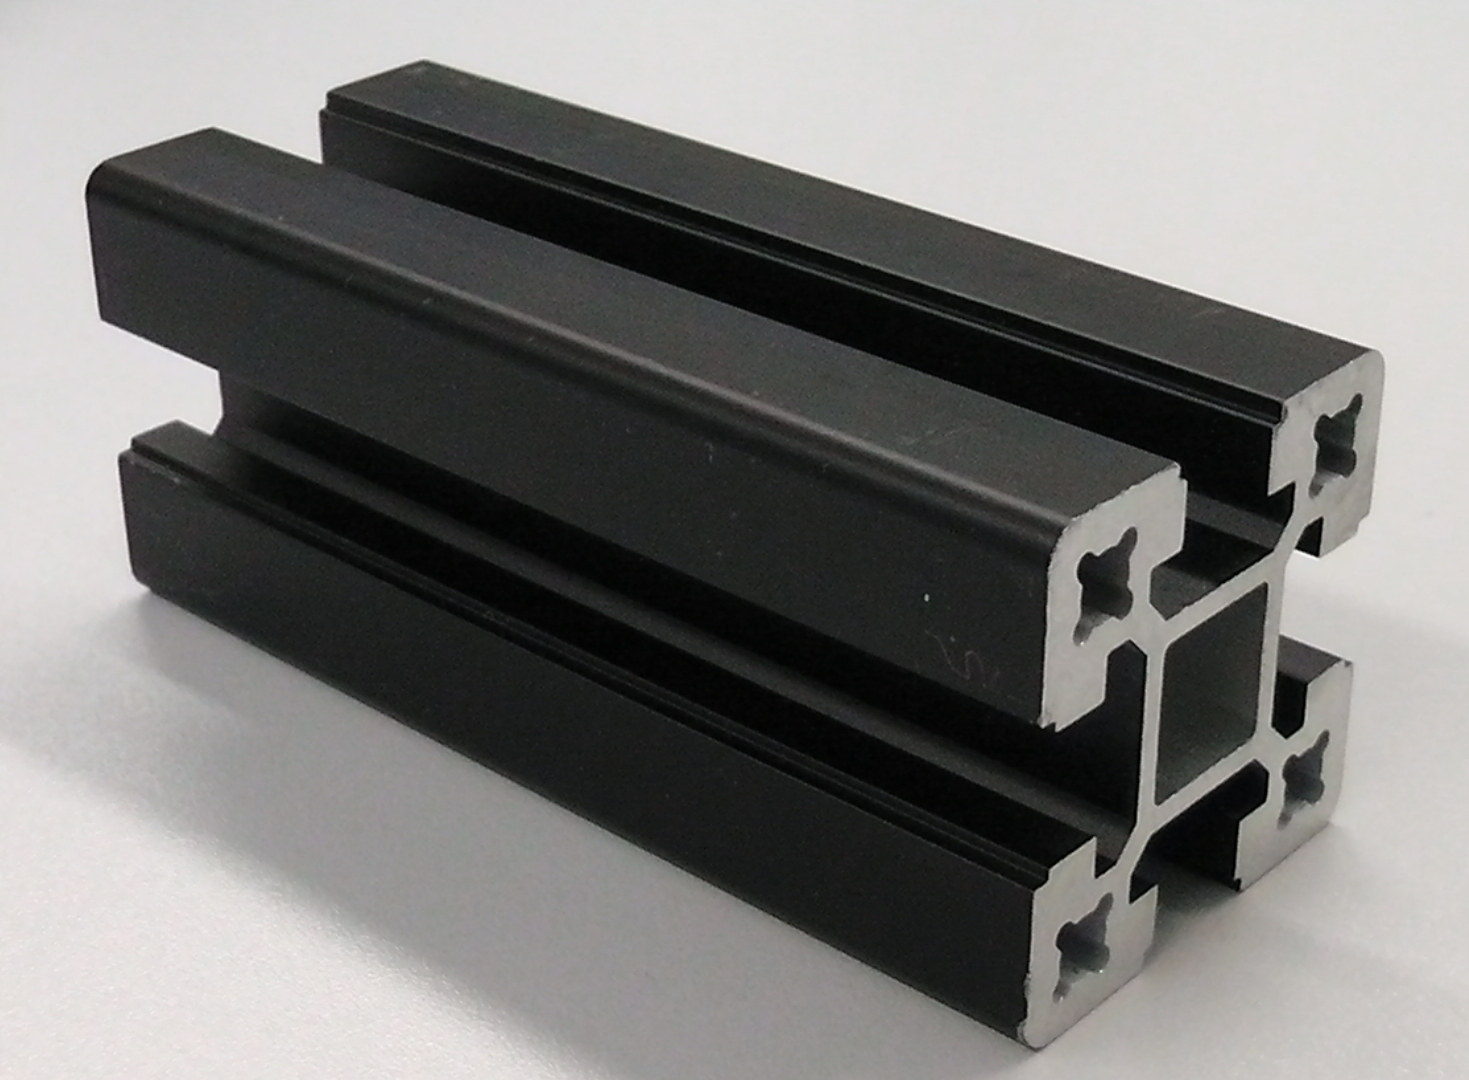
\includegraphics[width=.5\linewidth]{S40_40_B}
  \caption{S40\_40\_B \cite{github_robocup@work}}
  \label{fig:S40_40_B}
\end{subfigure}\\
\vspace{3mm}
\begin{subfigure}{.3\textwidth}
  \centering
  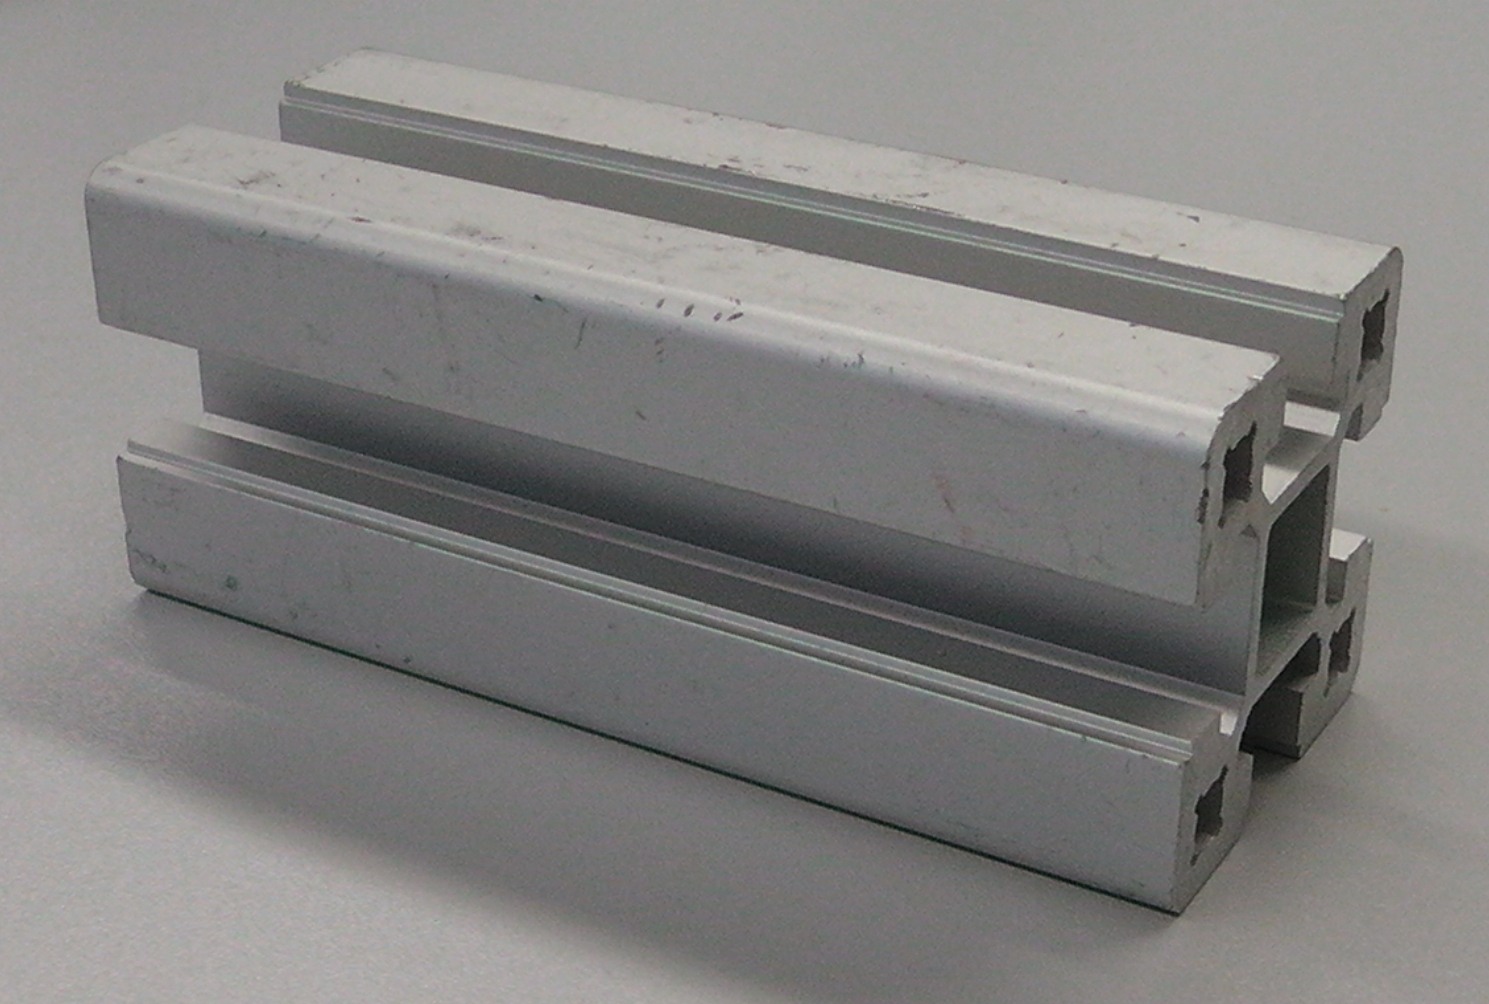
\includegraphics[width=.5\linewidth]{S40_40_G}
  \caption{S40\_40\_G \cite{github_robocup@work}}
  \label{fig:S40_40_G}
\end{subfigure}
\begin{subfigure}{.3\textwidth}
  \centering
  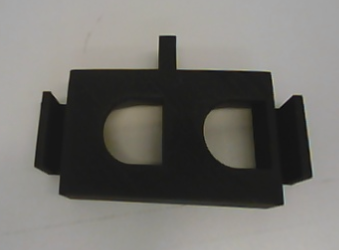
\includegraphics[width=.5\linewidth]{em_01}
  \caption{em\_01}
  \label{fig:em_01}
\end{subfigure}
\begin{subfigure}{.3\textwidth}
  \centering
  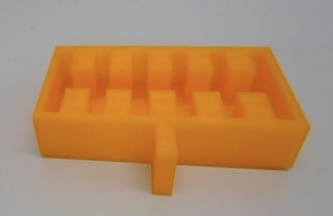
\includegraphics[width=.5\linewidth]{em_02}
  \caption{em\_02}
  \label{fig:em_02}
\end{subfigure}
\caption{Different objects required in the dataset}
\label{Fig:1}
\end{figure}

Each of the objects were taken individually, placed on 3 different backgrounds and 30 images were taken. This lead to a total of 540 images which were to be manually labeled. Since, every pixel of the images needs to be labeled, the process of manual annotation would be time consuming. Therefore, a decision was made to first annotate the 540 images and later decide whether more images could be taken based on the effort required for annotation.

\section{Selection of a labeling tool}
In order to reduce the time required to annotate an image, it was imperative to select a tool which is specifically designed for semantic segmentation and also provides algorithms which helps the annotator by providing labeling automation to the highest possible extent.

The following available tools were evaluated for ease of use and time taken for annotation:
	\begin{itemize}
		\item LabelMe: web based tool is public and data would also be public.
		\item LabelMe Matlab toolbox: yet to try..
		\item University bonn annotation tool:
		\item Pixel annotation tool (using watershed algorithm): works in windows. Seems to be useful.
		\item Ratsnake: tool dint seem to be useful although the website had options like superpixel suggestions.
		\item LabelImg: Can be used but time consuming.
		\item Figi: used in medical image segmentation. Has many options. Still exploring.
		\item Supervisely.
		\item MATLAB ImageLabeler available in release R2017b (Computer Vision Toolbox).
	\end{itemize}

\section{Description of the labeling process}
\label{section:process}
MATLAB ImageLabeler was used for the labeling process. At first, label definitions are created and exported to a .mat file. This file is used to load label definitions for all images to maintain consistency of labels. The contents of the .mat file is shown in the figure\ref{Fig:2}.

	\begin{figure}[htb!]
		\centering
		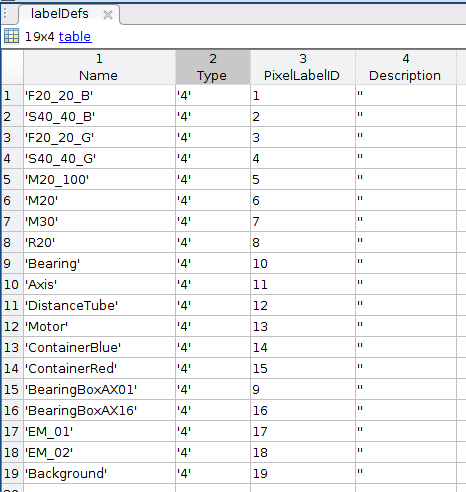
\includegraphics[scale=0.7]{labelDef}
		\caption{Contents of the labelDefs .mat file}
		\label{Fig:2}
	\end{figure}
	
The ImageLabeler app, by default, provides different tools which help create pixelwise labels\ref{Fig:3}. These tools become accessible once an image and the label definitions are loaded. A short description of the tools is given below:
	\begin{figure}[htb!]
		\centering
		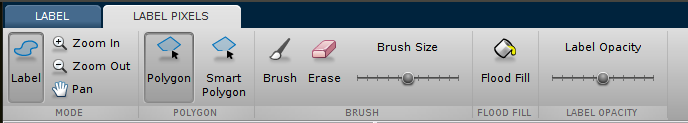
\includegraphics[scale=0.55]{label_tools}
		\caption{Tools provided by the ImageLabeler app}
		\label{Fig:3}
	\end{figure}
	
	\begin{itemize}
		\item Polygon: This can be used to trace an object boundary by placing dots. Once a closed contour is created, pixels within the contour get assigned the corresponding object label.
		\item Smart Polygon: Can be used in a similar fashion like the Polygon tool. This tool, in addition, tries to reach out to the nearby edges of the drawn polygon.
		\item Brush and Erase: Square shaped brush and eraser to either label a region or remove labels from a region. The size of the square can be changed by using the Brush Size slider.
		\item Flood Fill: This tool provides same labels to pixels which are similar in terms of the intensity with the selected pixel.
		\item Label Opacity: This tool provides a sliding bar which varies the opacity of the overlayed labels on the image. This is helpful to visualize the assigned labels.
		\item Zoom In, Zoom Out, Pan: These tools improve the ease of labeling by providing means to focus on particular regions by zooming and panning.
	\end{itemize}
	
The ImageLabeler app by default assigns different colors to different objects to aid visualization. The label colors are shown in the ROI Label Definition window\ref{Fig:4}.
	\begin{figure}[htb!]
		\centering
		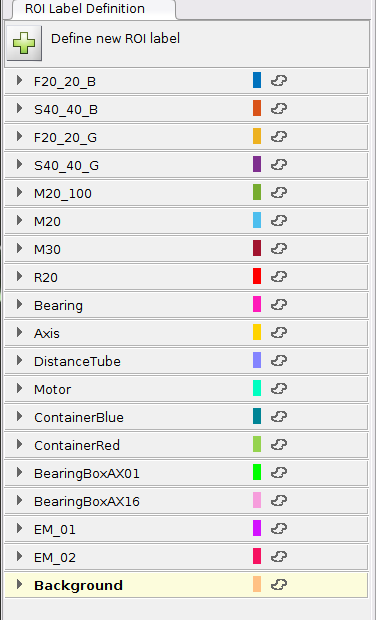
\includegraphics[scale=0.6]{roi_label_defintions}
		\caption{ROI Label Definitions window}
		\label{Fig:4}
	\end{figure}
	
The ImageLabeler app does not provide any tool to label all unlabeled pixels as background. In order to save time, the following workarounds have been used:
	\begin{itemize}
		\item The images taken for the dataset each have only one object in them.
		\item Only the object region is labeled.
		\item Since the ImageLabeler app does not provide any tool to label all unlabeled pixels as background, a python code which simply reads the label image and replaces unlabeled values 0 with background label value 19, was used for this purpose. The code is also used to double check the label image in order to avoid noisy labeling.
	\end{itemize}
	
The Export Labels -> To File option can be used to save the annotations. This is done for all images individually to arrive at the folder structure shown in \ref{Fig:5a}.
	
The saved .mat file can be loaded into ImageLabeler again to further modify labels if required later. The 'Label\_1.png' file located in the PixelLabelData folder (as can be seen in \ref{Fig:5a}) is the label image. This image is renamed to have the same name as the image file and a folder structure as in \ref{Fig:5b} is created by using a python code.
	
\begin{center}
	\begin{figure}[!htb]
		\begin{subfigure}{.5\textwidth}
			\centering
			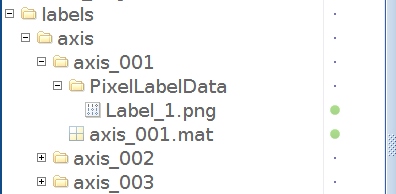
\includegraphics[width=1\linewidth]{folder_structure}
			\caption{Folder structure of saved labels}
			\label{Fig:5a}
		\end{subfigure}
		\begin{subfigure}{.5\textwidth}
			\centering
			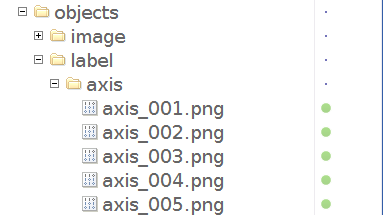
\includegraphics[width=1\linewidth]{folder_structure_aug}
			\caption{Rearranged folder structure}
			\label{Fig:5b}
		\end{subfigure}
		\caption{Different folder structures}
		\label{Fig:5}
	\end{figure}
\end{center}

The final folder structure is shown in \ref{Fig:6}. The image folder and label folder are similar and contain object images and corresponding label images with same names.

\begin{center}
	\begin{figure}[!htb]
		\begin{subfigure}{.5\textwidth}
			\centering
			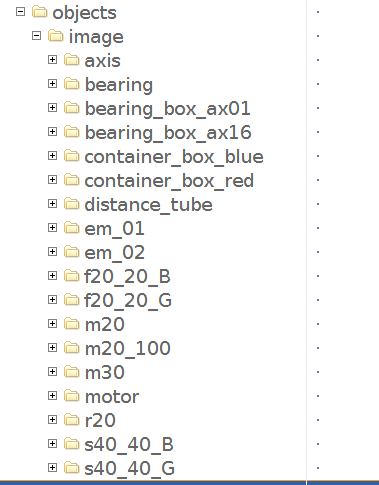
\includegraphics[width=1\linewidth]{folder_image}
			%\caption{}
			\label{Fig:6a}
		\end{subfigure}
		\begin{subfigure}{.5\textwidth}
			\centering
			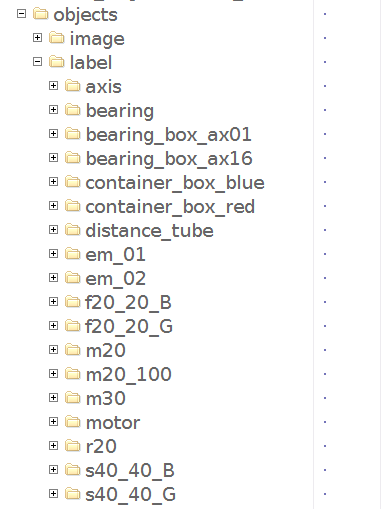
\includegraphics[width=1\linewidth]{folder_label}
			%\caption{}
			\label{Fig:6b}
		\end{subfigure}
		\caption{Folder structure showing different object folders in both image and label folders.}
		\label{Fig:6}
	\end{figure}
\end{center}

\section{About the augmentation algorithm}
\subsection{Motivation}
	\begin{itemize}
		\item Manually labeling 540 images with the described process in \ref{section:process} takes roughly 2160 minutes (roughly 4 minutes per image). This is equivalent to around 4 working days. Hence, creating a large dataset with manual labeling is not feasible.
		\item Taking images in a variety of real world backgrounds is also time consuming.
		\item Labeling images with multiple objects would take an even longer time.
	\end{itemize}
	
These drawbacks could be overcome by randomly placing objects on a variety of different background images automatically using an algorithm.

\subsection{Working}
The following steps are performed to result in the generation of augmented images:
	\begin{itemize}
	\label{List:1}
		\item[1] Given the path to the background images (for example, ''./backgrounds'), the images in the path are read and stored in a list.
		\item[2] Given the path to the 'image' folder (for example, './objects/image') and the 'label' folder (for example, './objects/label'), the algorithm fetches the paths of the label files and the corresponding paths of the image files. The number of label files available is also counted.
		\item[3] Each image and its corresponding label for each class of objects is read one by one. Different scales of the image and label for each image is also created based on the NUM\_OF\_SCALES keyword argument and added to an objects list. NUM\_OF\_SCALES argument can also be set to 'RANDOMIZE' in which case random number of scales in the range 1 to 5, will be used. If an added object is too small (determined using the MIN\_OBJ\_AREA\_PERCENT argument) or too big (determined using the MAX\_OBJ\_AREA\_PERCENT argument), it is removed from the list.
		\item[4] The list of objects contains the following details about each object:
			\begin{itemize}
				\item 'obj\_loc': The pixel locations of the object in the original image.
				\item 'obj\_vals': Intensity values of the object corresponding to 'obj\_loc'.
				\item 'label\_vals': Label values of the object corresponding to 'obj\_loc'.
				\item 'obj\_name': The name of the object.
				\item 'rect\_points': The top-left and bottom-right coordinates of the bounding rectangle of the object in pixel space.
				\item 'obj\_area': The area occupied by the object in pixel space.
			\end{itemize}
		An example is shown in the figure\ref{Fig:7}.
		\item[5] A list called 'augment\_vector' is created with each element denoting an augmented image, contains the following details.
			\begin{itemize}
				\item 'background\_image': A randomly choosen background image. It is also made sure that each available background is used atleast once before reselecting a background.
				\item 'num\_objects\_to\_place': Number of objects to be placed in the current augmented image.
				\item 'what\_objects': A list of random numbers which determines what objects from the objects list is selected.
				\item 'locations': A list of random locations in the pixel space where the selected objects need to be placed.
			\end{itemize}
		\item[6] Each of the elements in the augment\_vector is evaluated and elements whose objects occupy an area above MAX\_OCCUPIED\_AREA and whose object locations are too close to each other determined by MIN\_DIST\_BTW\_LOCATIONS, are removed.
		\item[7] A defined number of reattempts are made to regenerate the removed augment\_vectors. This number is set sufficiently high to obtain same number of augmented images as required by the user. However, it is possible that sometimes less number of images are generated because of the randomness invovled in the generation of augment\_vectors.
		\item[8] The elements in the augment\_vector are taken one by one and based on the taken element, objects are placed on the background. The resulting augmented image is saved in './data\_augmentation\_results/image/' and ground truth is saved in './data\_augmentation\_results/ground\_truth/'. Additionally object detection labels are also saved in csv files in the location './data\_augmentation\_results/obj\_det/'. A plot function is provided to visualize the labels and the visualized labels is also saved in './data\_augmentation\_results/image\_and\_gt/'.
	\end{itemize}
	
	\begin{figure}[htb!]
		\centering
		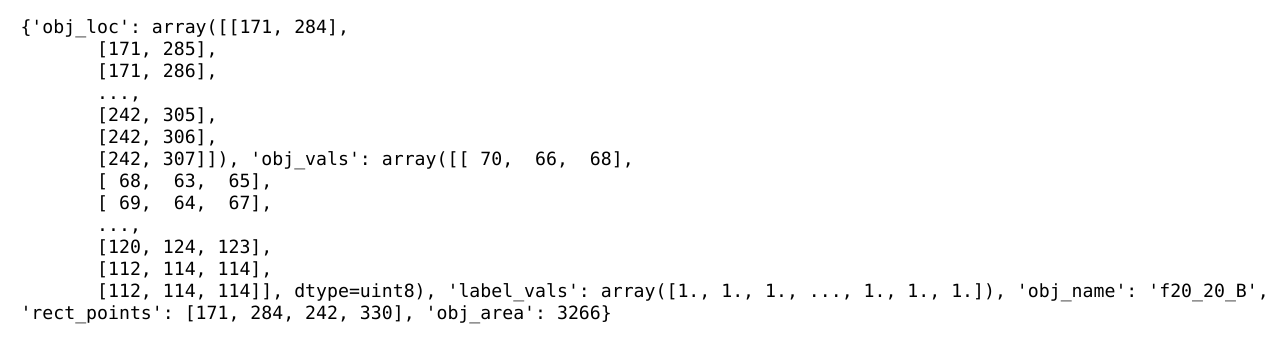
\includegraphics[scale=0.33]{obj_details}
		\caption{Details about an example object stored in the objects list}
		\label{Fig:7}
	\end{figure}
	
In \ref{List:1}, steps 1 to 4 are done by initializing the DataAugmentation class, steps 5 to 7 are done by calling the class method 'create\_augment\_vector' and step 8 is done by calling the class method 'perform\_augmentation'.
	
\subsection{Keyword arguments}

Details regarding the keyword arguments are provided in \ref{Table:1} and \ref{Table:2}. Apart from these arguments, a label definition dictionary containing the object names and corresponding label values needs to be created and passed as argument to the class initialization.

\begin{table}[!htb]
\centering
\begin{tabular}{|c|c|c|c|c|c|c|c|}
\hline 
\textbf{Keyword argument} & Description \\ 
\hline 
\textbf{IMAGE\_DIMENSION} & \makecell{The dimensions of the images in the dataset\\ can be changed using this parameter.} \\ 
\hline 
\textbf{NUM\_OF\_SCALES} & \makecell{Determines the scales of objects to be created\\ and added to the object list.} \\ 
\hline 
\textbf{BACKGROUNDS\_PATH} & \makecell{The path where the background files are located\\ can be set using this argument.} \\ 
\hline 
\textbf{IMAGE\_PATH} & \makecell{The path where the image files are located\\ can be set using this argument.} \\ 
\hline 
\textbf{LABEL\_PATH} & \makecell{The path where the label files are located\\ can be set using this argument.} \\ 
\hline 
\textbf{IMG\_TYPE} & \makecell{The extension type of the image \\files can be provided here.} \\ 
\hline 
\textbf{MIN\_OBJ\_AREA\_PERCENT} & \makecell{The minimum area an object should occupy \\ in the pixel space in percentage.} \\ 
\hline 
\textbf{MAX\_OBJ\_AREA\_PERCENT} & \makecell{The maximum area an object can occupy \\ in the pixel space in percentage.} \\ 
\hline 
\textbf{REMOVE\_CLUTTER} & \makecell{If set to true, augmented images with too \\ many objects and with objects which \\ are too close to each other are removed.} \\ 
\hline 
\textbf{NUM\_OF\_IMAGES} & \makecell{The number of augmented images required to be \\ generated can be set here.} \\ 
\hline  
\textbf{MAX\_OBJECTS\_PER\_IMAGE} & \makecell{The maximum number of objects which \\ are allowed in an augmented image.} \\ 
\hline 
\textbf{GENERATION\_REATTEMPTS} & \makecell{The number of reattempts which can be made \\ to regenerate removed augment vectors.} \\ 
\hline 
\textbf{CLEAR\_AUGMENT\_VECTOR} & \makecell{Can be used to clear generated augment vectors.} \\ 
\hline 
\textbf{MIN\_DIST\_BTW\_LOCATIONS} & \makecell{Minimum distance in terms of number of pixels \\ which can be allowed between two random locations \\ in an augmented image.} \\ 
\hline 
\textbf{MAX\_OCCUPIED\_AREA} & \makecell{The maximum area which can be occupied by all \\ the objects in the augment vector.} \\ 
\hline 
\textbf{PREVIEW\_DATA} & \makecell{If set to true, the generated objects and labels \\ are displayed inline in the jupyter notebook.} \\ 
\hline 
\textbf{SAVE\_DATA\_PREVIEW} & \makecell{If set to true, the generated visualization \\ plot for image and label is saved.} \\ 
\hline 
\textbf{GET\_OBJ\_DET\_LABEL} & \makecell{If set to true, object detection labels are saved.} \\ 
\hline 
\end{tabular}
\caption{Keyword Arguments Description} 
\label{Table:1}
\end{table}

\begin{table}[!htb]
%\centering
\begin{tabular}{|c|c|c|c|c|c|c|c|}
\hline 
\textbf{Keyword argument} & Default value & \makecell{DataAugmentation class \\ argument of method} \\ 
\hline 
\textbf{IMAGE\_DIMENSION} & [480, 640] & \makecell{\_\_init\_\_ method} \\ 
\hline 
\textbf{NUM\_OF\_SCALES} & 2 & \makecell{\_\_init\_\_ method} \\ 
\hline 
\textbf{BACKGROUNDS\_PATH} & './backgrounds' & \makecell{\_\_init\_\_ method} \\ 
\hline 
\textbf{IMAGE\_PATH} & './objects/image' & \makecell{\_\_init\_\_ method} \\ 
\hline 
\textbf{LABEL\_PATH} & './objects/label' & \makecell{\_\_init\_\_ method} \\ 
\hline 
\textbf{IMG\_TYPE} & '.jpg' & \makecell{\_\_init\_\_ method} \\ 
\hline 
\textbf{MIN\_OBJ\_AREA\_PERCENT} & 0.3 & \makecell{\_\_init\_\_ method} \\ 
\hline 
\textbf{MAX\_OBJ\_AREA\_PERCENT} & 70 & \makecell{\_\_init\_\_ method} \\ 
\hline 
\textbf{REMOVE\_CLUTTER} & True & \makecell{create\_augment\_vector \\ method} \\ 
\hline 
\textbf{NUM\_OF\_IMAGES} & 50 & \makecell{create\_augment\_vector \\ method} \\ 
\hline 
\textbf{MAX\_OBJECTS\_PER\_IMAGE} & 6 & \makecell{create\_augment\_vector \\ method} \\ 
\hline 
\textbf{GENERATION\_REATTEMPTS} & 100 & \makecell{create\_augment\_vector \\ method} \\ 
\hline 
\textbf{CLEAR\_AUGMENT\_VECTOR} & True & \makecell{create\_augment\_vector \\ method} \\ 
\hline 
\textbf{MIN\_DIST\_BTW\_LOCATIONS} & 70 & \makecell{create\_augment\_vector \\ method} \\ 
\hline 
\textbf{MAX\_OCCUPIED\_AREA} & 0.8 & \makecell{create\_augment\_vector \\ method} \\ 
\hline 
\textbf{PREVIEW\_DATA} & False & \makecell{perform\_augmentation \\ method} \\ 
\hline 
\textbf{SAVE\_DATA\_PREVIEW} & False & \makecell{perform\_augmentation \\ method} \\ 
\hline 
\textbf{GET\_OBJ\_DET\_LABEL} & True & \makecell{perform\_augmentation \\ method} \\ 
\hline 
\end{tabular}
\caption{Details regarding the keyword arguments}
\label{Table:2}
\end{table}

\subsection{Sample results}
Some sample results can be seen in \ref{Fig:8}. The yellow bounding box represents the object detection label and the different colors of the segmentation labels denote different label values.

	\begin{figure}[htb!]
		\centering
		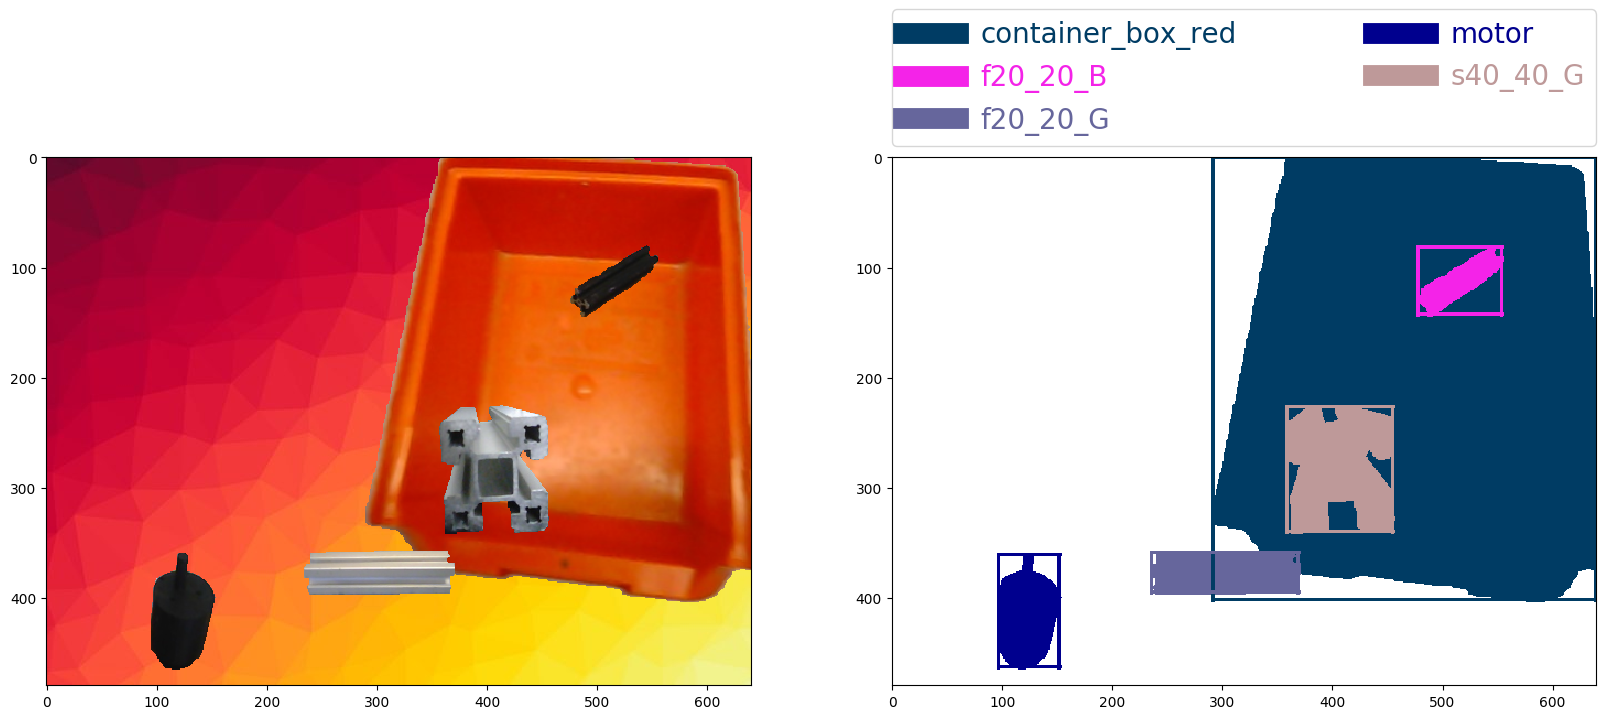
\includegraphics[scale=0.4]{sample_result_1}
		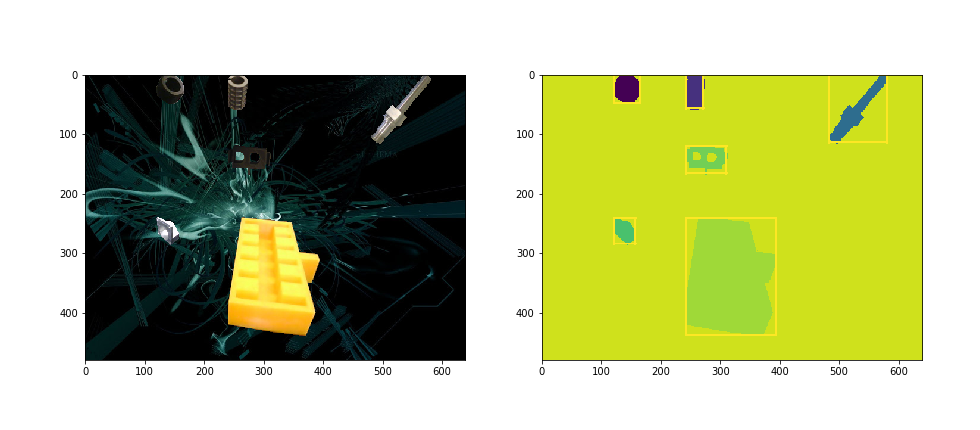
\includegraphics[scale=0.4]{sample_result_2}
		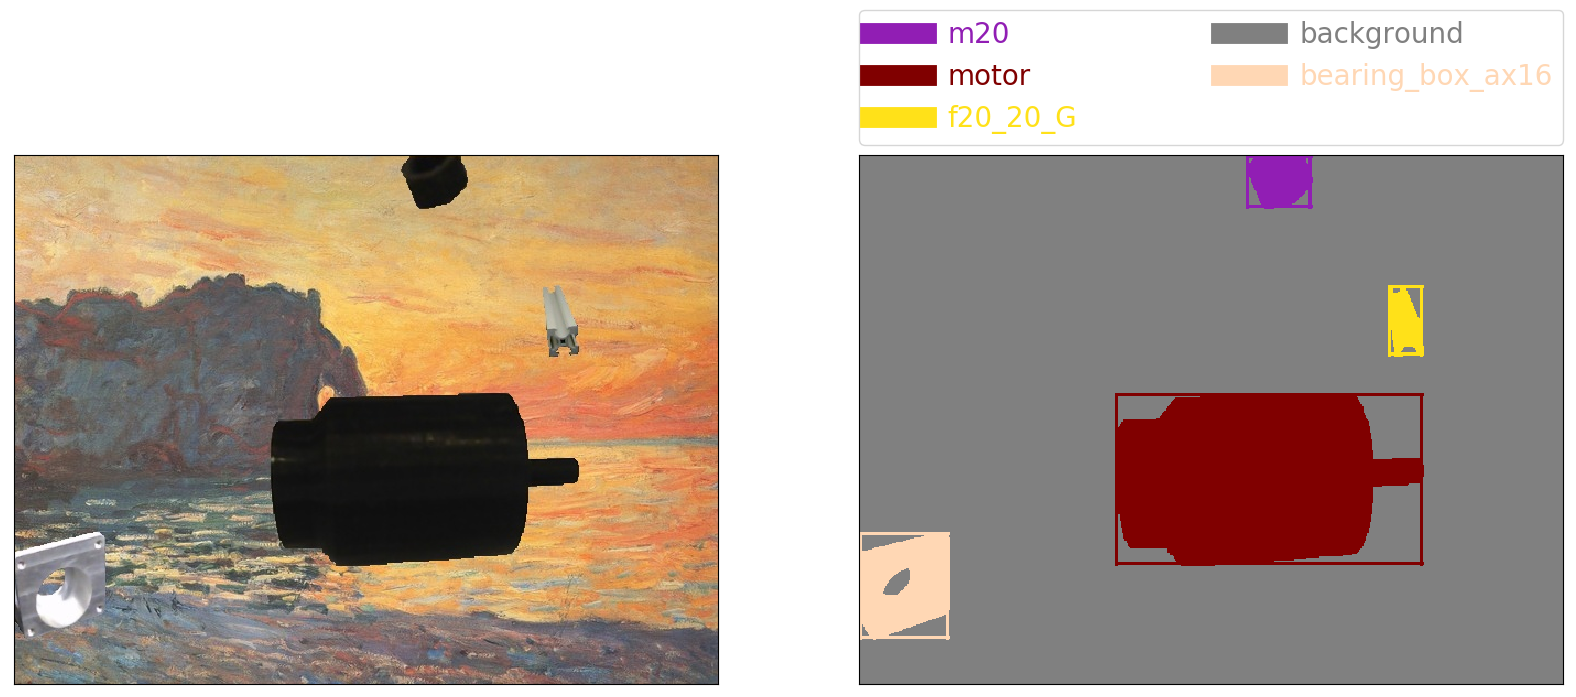
\includegraphics[scale=0.4]{sample_result_3}
		\caption{Sample results produced by the augmentation script}
		\label{Fig:8}
	\end{figure}
	

\section{Metadata of the dataset}

Details regarding the dataset is provided in table \ref{Table:3}.

\begin{table}[!htb]
\centering
\begin{tabular}{|c|c|c|c|c|c|c|c|}
\hline 
    & Training & Validation & Test \\ 
\hline 
Real Images & \makecell{30 per object.\\ Total: 30$\times$18=540} & \makecell{5 per object.\\ Total: 5$\times$18=90} & \makecell{5 per object.\\ Total: 5$\times$18=90} \\ 
\hline 
Augmented Images & 5000 & 810 & 810 \\ 
\hline 
Total Images & 5540 & 900 & 900 \\ 
\hline 
\end{tabular}
\caption{Metadata of the dataset} 
\label{Table:3}
\end{table}

\section{Conclusion and possible directions of improvement}

Creating a custom dataset for a desired application is evidently challenging. To overcome the time consuming nature of creating annotations for semantic segmentation, choices such as 1. placing just 1 object per image while taking real images and 2. augmenting the objects on a random selection of diverse backgrounds, were made. This method of augmentation, although inspired by dataset generation method used in \cite{DBLP:journals/corr/abs-1709-00849} and the Synthia dataset \cite{RosCVPR16}, takes a different approach. Unlike \cite{DBLP:journals/corr/abs-1709-00849}, which uses 3D CAD models, this approach does not require any 3D models. Also, this approach does not require a virtual world as used by the Synthia dataset \cite{RosCVPR16}. However, the effectiveness of the dataset is yet to be verified by training and testing available segmentation models.
The following list provides possible directions of improvement:
	\begin{itemize}
		\item The ImageLabeler app by default saves the label '.png' file with the name 'Label\_1.png' in a folder called PixelLabelData. A automation script can be written and added to the ImageLabeler to provide options to save the label file in a way the user wants.
		\item Creating a way to replace all unlabeled pixels with the label value of 'background' from within the ImageLabeler would be helpful. For now, this is done by first exporting the label, then loading the label using opencv in python to replace 0 (value of unlabeled pixels) with 19 (value of 'background').
		\item The augmentation script is written in python and is independent of the MATLAB ImageLabeler app. This can be improved by including a way to start augmentation right from the ImageLabeler.
		\item A GUI for the augmentation script can be created to improve the ease of use.
	\end{itemize}

\newpage
\addcontentsline{toc}{section}{References}

\bibliographystyle{plain}
\bibliography{references}
\end{document}
